\documentclass[10pt]{beamer}

% ------------------------------------------------------------------------
% Carga de tu preámbulo personalizado (preamble.tex)
% Asegúrate de tenerlo en la misma carpeta para que \input funcione.
% ------------------------------------------------------------------------
\usetheme[progressbar=frametitle]{metropolis}
\usepackage{appendixnumberbeamer}
\usepackage{fancyvrb}
\usepackage{booktabs}
\usepackage[scale=2]{ccicons}
\usepackage{pgfplots}
\usepgfplotslibrary{dateplot}
\usepackage{type1cm}
\usepackage{lettrine}
\usepackage{ragged2e}
\usepackage{xspace}
\newcommand{\themename}{\textbf{\textsc{metropolis}}\xspace}
\usepackage{graphicx} % Allows including images
\usepackage{booktabs} % Allows the use of \toprule, \midrule and \bottomrule in tables
\usepackage[utf8]{inputenc} %solucion del problema de los acentos.
\usepackage{xcolor}
\definecolor{LightGray}{gray}{0.9}

\usepackage{minted}
\usemintedstyle{tango}
\newcommand{\mypyfile}[1]{\inputminted[linenos=true, fontsize=\footnotesize, frame=lines, framesep=5\fboxrule,framerule=1pt]{python}{#1}}

\setminted[python]{breaklines,frame=lines,framesep=2mm,baselinestretch=1.2,bgcolor=LightGray,linenos, fontsize=\footnotesize} % obeytabs=true, tabsize=2, showtabs=true}

%%%%%%%%%%%%%%%%%%%%%%%%%%%%%%%%%%%%%%%%%%%%%%%%%%%%%%%%%%%%%%%%%%%%%%%%%%%%%%%%%%%%%%
\setbeamercolor{progress bar}{fg=blue!50!black,bg=white!50!black}
\setbeamercolor{title separator}{fg=red!50!black,bg=white!50!black}
\setbeamercolor{frametitle}{fg=white!80!black,bg=red!50!black}
\title[PCFI161]{Programaci\'on para F\'isica y Astronom\'ia}
\subtitle{Departamento de Física.}

\newcommand{\myfront}{
\author[PCFI161]{Corodinadora: C Loyola \\ Profesoras/es C Loyola / C Femenías / Y Navarrete / C Ruiz}
\institute[UNAB]{Universidad Andrés Bello}
\date{Primer Semestre 2025}
}

\titlegraphic{%
  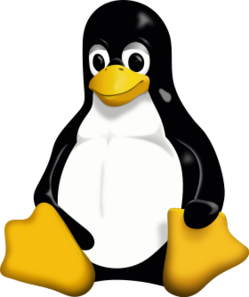
\includegraphics[width=.08\textwidth]{logo-tux.png}\hfill
  
\includegraphics[width=.3\textwidth]{logo-unab.png}\hfill
  
\includegraphics[width=.08\textwidth]{logo-python.png}
}

\makeatletter
\setbeamertemplate{title page}{
  \begin{minipage}[b][\paperheight]{\textwidth}
    \vfill%
    \ifx\inserttitle\@empty\else\usebeamertemplate*{title}\fi
    \ifx\insertsubtitle\@empty\else\usebeamertemplate*{subtitle}\fi
    \usebeamertemplate*{title separator}
    \ifx\beamer@shortauthor\@empty\else\usebeamertemplate*{author}\fi
    \ifx\insertdate\@empty\else\usebeamertemplate*{date}\fi
    \ifx\insertinstitute\@empty\else\usebeamertemplate*{institute}\fi
    \vfill
    \ifx\inserttitlegraphic\@empty\else\inserttitlegraphic\fi
    \vspace*{1cm}
  \end{minipage}
}
\makeatother


\makeatletter
\setlength{\metropolis@titleseparator@linewidth}{2pt}
\setlength{\metropolis@progressonsectionpage@linewidth}{2pt}
\setlength{\metropolis@progressinheadfoot@linewidth}{2pt}
\makeatother


\begin{document}

% ------------------------------------------------------------------------
% Portada personalizada (ejemplo \myfront si está definido en tu preámbulo)
% ------------------------------------------------------------------------
\myfront{}

% ------------------------------------------------------------------------
% Slide 1: Título de la Sesión
% ------------------------------------------------------------------------
\begin{frame}
  \titlepage
  % Por ejemplo:
  % \title{Semana 4 - Sesión 2 (Sesión 8): Taller de Funciones, Módulos y Librerías Externas}
\end{frame}

% ------------------------------------------------------------------------
% Slide 2: Índice / Tabla de Contenidos
% ------------------------------------------------------------------------
\begin{frame}
  \frametitle{Resumen - Semana 4, Sesión 2 (Sesión 8)}
  \tableofcontents
\end{frame}

% ----------------------------------------------------------------------------------------
% SECCIÓN 1: Introducción y Repaso de la Sesión Anterior
% ----------------------------------------------------------------------------------------
\section{Repaso y Contexto}

% ------------------------------------------------------------------------
% Slide 3: Repaso de las semanas previas y conexión con la sesión actual
% ------------------------------------------------------------------------
\begin{frame}{Repaso de Semanas Previas}
  \begin{itemize}
    \item \textbf{Semana 1:} Sintaxis básica, variables, tipos de datos y operadores.
    \item \textbf{Semana 2:} Estructuras de control: condicionales (\texttt{if-elif-else}), bucles (\texttt{for}, \texttt{while}).
    \item \textbf{Semana 3:} Definición y uso de funciones, alcance de variables, introducción a módulos.
    \item \textbf{Conexión:} Todos estos conceptos se integran en la sesión de hoy para crear aplicaciones más estructuradas y reutilizables.
  \end{itemize}
  \begin{block}{Ejemplo de integración}
    Un programa que calcula el área de figuras, valida datos y organiza el código en funciones y módulos.
  \end{block}
\end{frame}

% ------------------------------------------------------------------------
% Slide 4: Objetivos de la Sesión
% ------------------------------------------------------------------------
\begin{frame}{Objetivos de la Sesión}
  \begin{itemize}
    \item \textbf{Integrar} variables, operadores, estructuras de control y funciones en ejercicios prácticos.
    \item \textbf{Aplicar} la modularización mediante la creación y uso de módulos propios.
    \item \textbf{Desarrollar} habilidades para resolver problemas físicos y matemáticos usando Python.
    \item \textbf{Preparar} el terreno para proyectos colaborativos y el uso de paquetes externos.
  \end{itemize}
\end{frame}


\section{Ejercicios Prácticos Integrados}

% -------------------- Ejercicios Intermedios --------------------

% Ejercicio 1 (Intermedio)
\begin{frame}{Ejercicio 1: \hfill \textcolor{red}{$\clubsuit$} \\ Suma de números pares en un rango}
  \begin{block}{Enunciado}
    \begin{itemize}
      \item Solicita dos números enteros, inicio y fin.
      \item Calcula la suma de todos los números pares en ese rango usando un bucle.
      \item Muestra el resultado.
    \end{itemize}
  \end{block}
  \textbf{Conceptos:} Bucles, condicionales, operadores.\\
  \textbf{Física relevante:} Lógica computacional.
\end{frame}

% Ejercicio 2 (Intermedio)
\begin{frame}{Ejercicio 2: \hfill \textcolor{red}{$\clubsuit$} \\ Validación de entrada para masa positiva}
  \begin{block}{Enunciado}
    \begin{itemize}
      \item Solicita la masa de un objeto (kg).
      \item Si la masa es negativa o cero, vuelve a pedir el dato hasta que sea válido.
      \item Muestra la masa final.
    \end{itemize}
  \end{block}
  \textbf{Conceptos:} Bucles (\texttt{while}), validación de datos.\\
  \textbf{Física relevante:} Medición y control de errores.
\end{frame}

% Ejercicio 3 (Intermedio)
\begin{frame}{Ejercicio 3: \hfill \textcolor{red}{$\clubsuit$} \\ Conversión de lista de temperaturas}
  \begin{block}{Enunciado}
    \begin{itemize}
      \item Solicita una lista de temperaturas en Celsius separadas por comas.
      \item Convierte cada valor a Fahrenheit y muestra la lista convertida.
    \end{itemize}
  \end{block}
  \textbf{Conceptos:} Listas, bucles, operadores.\\
  \textbf{Física relevante:} Termodinámica básica.
\end{frame}

% Ejercicio 4 (Intermedio)
\begin{frame}{Ejercicio 4: \hfill \textcolor{red}{$\clubsuit$} \\ Cálculo de energía potencial gravitatoria}
  \begin{block}{Enunciado}
    \begin{itemize}
      \item Solicita masa (kg) y altura (m).
      \item Calcula la energía potencial: \(E_p = mgh\), con \(g = 9.8\,m/s^2\).
      \item Usa una función para el cálculo y muestra el resultado.
    \end{itemize}
  \end{block}
  \textbf{Conceptos:} Funciones, operadores, entrada/salida.\\
  \textbf{Física relevante:} Mecánica clásica.
\end{frame}

% Ejercicio 5 (Intermedio)
\begin{frame}{Ejercicio 5: \hfill \textcolor{red}{$\clubsuit$} \\ Tabla de conversión de segundos a horas}
  \begin{block}{Enunciado}
    \begin{itemize}
      \item Solicita un número entero \(n\).
      \item Imprime una tabla de conversión de los primeros \(n\) valores (1 a \(n\)) de segundos a horas.
    \end{itemize}
  \end{block}
  \textbf{Conceptos:} Bucles (\texttt{for}), operadores, entrada/salida.\\
  \textbf{Física relevante:} Unidades y conversiones.
\end{frame}

% -------------------- Ejercicios Difíciles --------------------

% Ejercicio 6 (Difícil)
\begin{frame}{Ejercicio 6: \hfill \textcolor{red}{$\clubsuit$} \\ Módulo de conversiones físicas avanzadas}
  \begin{block}{Enunciado}
    \begin{itemize}
      \item Crea un módulo \texttt{conversor.py} con funciones para convertir:
        \begin{itemize}
          \item Newtons a kilogramos-fuerza.
          \item Joules a calorías.
          \item Pascales a atmósferas.
        \end{itemize}
      \item Importa el módulo y prueba cada función.
    \end{itemize}
  \end{block}
  \textbf{Conceptos:} Módulos, funciones, importación.\\
  \textbf{Física relevante:} Unidades físicas avanzadas.
\end{frame}

% ------------------------------------------------------------------------
% Ejercicio 7 (Intermedio)
% ------------------------------------------------------------------------
\begin{frame}{Ejercicio 7: \hfill \textcolor{red}{$\clubsuit$} \\ Validación y suma de números positivos}
  \begin{block}{Enunciado}
    \begin{itemize}
      \item Crea una función que solicite al usuario ingresar 5 números.
      \item Si el número ingresado es negativo, vuelve a pedirlo hasta que sea positivo.
      \item Al final, muestra la suma total de los números ingresados.
    \end{itemize}
  \end{block}
  \textbf{Conceptos:} Funciones, bucle \texttt{while}, validación de datos, acumuladores.\\
  \textbf{Física relevante:} Control de errores en mediciones.
\end{frame}

% ------------------------------------------------------------------------
% Ejercicio 8 (Difícil)
% ------------------------------------------------------------------------
\begin{frame}{Ejercicio 8: \hfill \textcolor{red}{$\clubsuit$} \\ Aproximación de la raíz cuadrada por método iterativo}
  \begin{block}{Enunciado}
    \begin{itemize}
      \item Crea una función que solicite un número positivo.
      \item Calcula la raíz cuadrada usando el método de Newton-Raphson:
        \[
        x_{n+1} = \frac{1}{2}\left(x_n + \frac{a}{x_n}\right)
        \]
        donde \(a\) es el número ingresado y \(x_0 = a/2\).
      \item Usa un ciclo \texttt{for} para realizar 10 iteraciones y muestra el resultado final.
    \end{itemize}
  \end{block}
  \textbf{Conceptos:} Funciones, ciclo \texttt{for}, aproximación numérica, operadores.\\
  \textbf{Física relevante:} Métodos numéricos aplicados a física.
\end{frame}



% Ejercicio 9 (Difícil)
\begin{frame}{Ejercicio 9: \hfill \textcolor{red}{$\clubsuit$} \\ Generador de tabla de valores de una función física}
  \begin{block}{Enunciado}
    \begin{itemize}
      \item Imprime una tabla de una ecuacion (por ejemplo, \(y = v_0 t - \frac{1}{2}gt^2\)), 
      \item Pide los valores iniciales \(v_0\) y  \(t_f\), teniendo encuenta que \(t_0 = 0 \).
      \item Imprime una tabla con los valores calculados (por ejemplo, \(y\) para diferentes valores de \(t\)).
    \end{itemize}
  \end{block}
  \textbf{Conceptos:} Bucles, operadores, entrada/salida, funciones.\\
  \textbf{Física relevante:} Movimiento rectilíneo uniformemente acelerado.
\end{frame}

% ------------------------------------------------------------------------
% Ejercicio 10 (Difícil)
% ------------------------------------------------------------------------
\begin{frame}{Ejercicio 10: \hfill \textcolor{red}{$\clubsuit$} \\ Simulación de crecimiento poblacional}
  \begin{block}{Enunciado}
    \begin{itemize}
      \item Crea una función que solicite la población inicial, la tasa de crecimiento porcentual anual y el número de años.
      \item Usa la fórmula de crecimiento exponencial:
        \[
        P_{n} = P_0 \times (1 + r)^n
        \]
        donde \(P_0\) es la población inicial, \(r\) es la tasa de crecimiento (como decimal), y \(n\) es el número de años.
      \item Usa un ciclo \texttt{for} para calcular y mostrar la población para cada año.
    \end{itemize}
  \end{block}
  \textbf{Conceptos:} Funciones, ciclo \texttt{for}, operadores, entrada/salida.\\
  \textbf{Física relevante:} Modelos matemáticos en biología y física.
\end{frame}


\section{Conclusiones}


% ------------------------------------------------------------------------
% Slide 23: Síntesis y Reflexión Final
% ------------------------------------------------------------------------
\begin{frame}{Síntesis de la Sesión}
  \begin{itemize}
    \item \textbf{Consolidamos:} el uso integrado de variables, operadores, condicionales, bucles y funciones.
    \item \textbf{Aplicamos:} la modularización y reutilización del código mediante módulos propios.
    \item \textbf{Resolvimos:} problemas físicos y matemáticos con Python, conectando teoría y práctica.
    \item \textbf{Preparamos:} el camino para el trabajo colaborativo y el uso de librerías externas.
  \end{itemize}
  \begin{block}{Habilidad adquirida}
    Capacidad para estructurar programas en Python de forma clara, eficiente y reutilizable.
  \end{block}
\end{frame}


% ------------------------------------------------------------------------
% Slide 25: Cierre y Motivación
% ------------------------------------------------------------------------
\begin{frame}
  \huge{\centerline{¡Excelente trabajo!}}
  \vspace{0.5cm}
  \normalsize
  \begin{itemize}
    \item Guarda tus avances y comparte dudas en el foro.
    \item Explora la documentación oficial de Python y experimenta con nuevos módulos.
    \item ¡Sigue practicando y colaborando!
  \end{itemize}
\end{frame}

\end{document}

